%%%%%%%%%%%%%%%%%%%%%%%%%%%%%%%%%%%
\subsection{Cameras}
\label{sec:fdgen-slow-cryo-cameras}
% glenn, jim s, chuck
% same text in single and dual phase

Cameras provide direct visual information about the state of the
\dword{detmodule} during critical operations and when damage or unusual
conditions are suspected.  Cameras in the \dword{wa105} allowed spray from cool-down
nozzles to be seen, and the level and state of the \lar to be
observed as it covered the \dword{crp} \cite{Murphy:20170516}.  A camera was
used in the Liquid Argon Purity Demonstrator
cryostat\cite{Adamowski:2014daa} to study \dword{hv} discharges in
\lar, and in EXO-100 during operation of a TPC
\cite{Delaquis:2013hva}.  Warm cameras viewing \lar from a distance
have been used to observe \dword{hv} discharges in \lar in
fine detail \cite{Auger:2015xlo}.  Cameras are commonly used during
calibration source deployment in many experiments ({\em e.g.,} the
\kamland ultra-clean system \cite{Banks:2014hra}).

In DUNE, cameras are used to verify the stability, straightness,
and alignment of the hanging TPC structures during cool-down and
filling; to ensure that there is no bubbling near the \dwords{gp}
(\single) or \dwords{crp} (\dual); to inspect the
state of movable parts in the \dword{detmodule} (calibration devices, dynamic
thermometers) as needed; and to closely inspect parts of the TPC as
necessary following any seismic activity or other unanticipated
occurrence.  These functions are performed using set of fixed
\textit{cold} cameras permanently mounted at fixed points in the cryostat
for use during filling and commissioning, and a movable, replaceable
\textit{warm} inspection camera that can be deployed through any free
instrumentation flange at any time throughout the life of the
experiment.  Table \ref{tab:fdgen-cameras-req} summarizes the
requirements for the camera system.

\begin{dunetable}
[Camera system Requirements]
{p{0.45\linewidth}p{0.50\linewidth}}
{tab:fdgen-cameras-req}
{Camera system requirements}   
 Requirement & Physics Requirement Driver \\ \toprowrule
 {\bf General} \\ \colhline
 No component may contaminate the \lar{}. & High \lar purity is required for TPC operation. \\ \toprowrule
 No component may produce bubbles in the liquid argon if the \dword{hv} is on. & Bubbles increase risk of \dword{hv} discharge. \\ \toprowrule
 No point in the camera system shall have a field greater than \SI{15}{kV/cm} when the drift field is at nominal voltage. & Fields must be well below \SI{30}{kV/cm} to avoid risk of \dword{hv} discharge.\\ \toprowrule
The camera system shall not produce measurable noise in any detector system. & Low noise is required for TPC operation. \\ \toprowrule
 Cameras provide the viewing functionality as agreed upon with the other subsystems for viewing, as documented in the ICDs with the individual systems. \\ \toprowrule
{\bf Cold cameras} \\ \colhline
minimal heat dissipation when camera not in operation & do not generate bubbles when \dword{hv} is on \\ \colhline
longevity exceeds 18 months & cameras must function throughout cryostat filling and detector commissioning \\ \colhline
Frame rate \(\geq\SI{10}{\per s}\) & observe bubbling, waves, detritus, etc. \\ \colhline
{\bf Inspection cameras} \\ \colhline
low heat transfer to \lar when in operation & do not generate bubbles, some use cases may require operation when \dword{hv} is on \\ \colhline
deployable without exposing \lar to air & keep \lar free N2 and other electronegative contaminants \\ \colhline
replaceable camera enclosure & replace broken camera, or upgrade, throughout life of experiment \\ \colhline
{\bf Light emitting system} \\ \colhline
no emitted wavelength shorter than \(\SI{400}{nm}\) & avoid damaging \dword{tpb} waveshifter \\ \colhline
longevity exceeds \num{18} months & lighting for fixed cameras must function throughout cryostat filling and detector commissioning \\ \colhline
\end{dunetable}


The following sections describe the design considerations for the cold
and warm cameras and the associated lighting system.  The same basic
design may be used for both the single and dual phase detectors.



% % % %
\subsubsection{Cryogenic Cameras (Cold)}

The fixed cameras %will be used to 
monitor the following items during filling:
\begin{itemize}
\item Positions of corners of \dword{apa} or \dword{crp}, \dword{cpa} or cathode, \dwords{fc}, \dwords{gp} (\SI{1}{mm} resolution);
\item Relative straightness and alignment of \dword{apa}/\dword{crp}, \dword{cpa}/cathode, and \dword{fc} (\(<\sim\SI{1}{mm}\));
\item Relative position of profiles and endcaps (\SI{0.5}{mm} resolution);
\item State of \lar surface: i.e., bubbling, debris.
\end{itemize}

There are published articles and unpublished presentations describing
completely or partially successful operation of low-cost,
off-the-shelf \dword{cmos} cameras in custom enclosures immersed in cryogens.
(e.g., EXO-100: \cite{Delaquis:2013hva}; DUNE \dword{35t} test
\cite{McConkey:2016spe}; \dword{wa105}: \cite{Murphy:20170516}.)  Generally
it is reported that such cameras show poor performance and ultimately
fail to function below some temperature of order \SIrange{150}{200}{K}, but some report that their cameras recover fully after
being stored (not operated) at temperatures as low as \SI{77}{K} and
then brought up to minimum operating temperature.

However, as with photon sensors, experience has also shown that it is
non-trivial to ensure reliable and reproducible mechanical and
electrical integrity of such cameras in the cryogenic environment.
({\em E.g.}, \cite{McConkey:2016spe} and
\cite{Valencia-Rodriquez:20180130}.)  Off-the-shelf cameras and camera
components are generally only specified by the vendors and original
manufacturers for operation down to \SI{-40}{\celsius} or \SI{-50}{\celsius}.
In addition, many low-cost cameras use digital interfaces not intended
for long distance deployment, such as USB (\(2\sim\SI{5}{m}\)) or CSI (circuit
board scale), leading to signal degradation and noise problems.

The design for the DUNE fixed cameras uses an enclosure based on
the successful EXO-100 design\cite{Delaquis:2013hva}, which was also
used successfully in
LAPD. (See Figure~ref{fig:gen-fdgen-cameras-enclosure}) The enclosure is
 connected to a stainless steel gas line to allow the enclosure to be
flushed with argon gas at low enough pressure to prevent
liquification, using the same design asthe gas line for the beam plug
tested in the \dword{35t} \dword{hv} test and in \dword{protodune}.  A thermocouple in the
enclosure allows temperature monitoring, and a heating element
provides temperature control.  The camera transmits its video
signal using either a composite video signal over shielded coax or
Ethernet over optical fiber.  Most importantly, the DUNE \dword{cisc}
consortium must work with vendors to design camera circuit boards that
are robust and reliable in the cryogenic environment.

\begin{dunefigure}[A camera enclosure]{fig:gen-fdgen-cameras-enclosure}
  {CAD exploded view of vacuum-tight camera enclosure suited for cryogenic applications from \cite{Delaquis:2013hva}.
    (1) quartz window, (2 and 7) copper gasket, (3 and 6) flanges, (4) indium wires, (5) body piece, (8) signal \fdth.
  }
  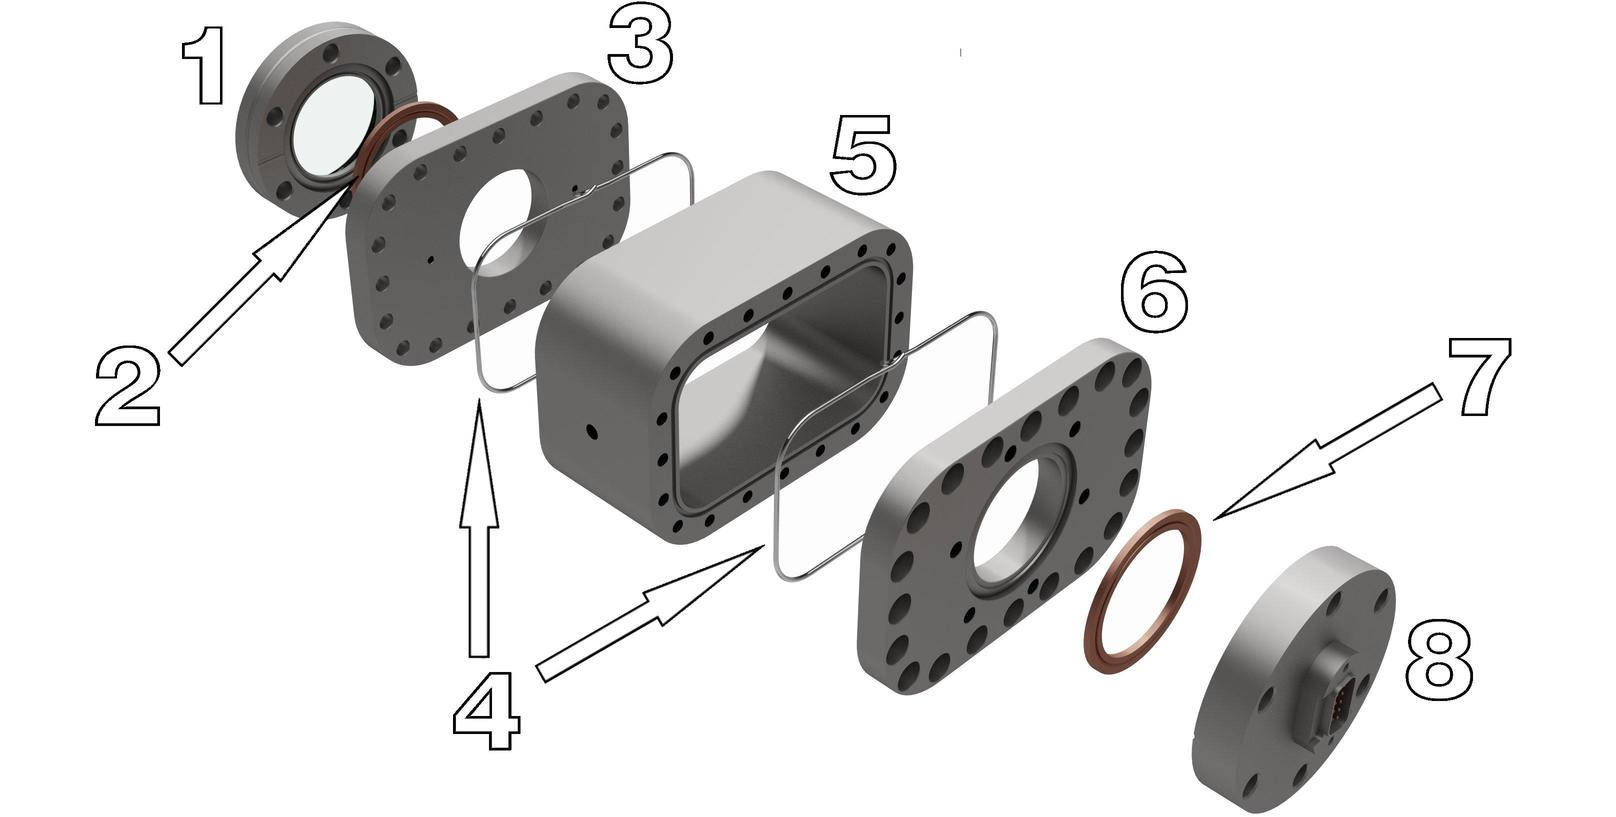
\includegraphics[width=0.6\textwidth]{exo100-camera-case}%
\end{dunefigure}



% % % %
\subsubsection{Inspection Cameras (Warm)}

The inspection cameras are intended to be as versatile as possible.
However, the following locations have been identified as likely
to be of interest:
\begin{itemize}
\item Status of \dword{hv} \fdth and cup;
\item Status of \dword{fc} profiles, endcaps (\SI{0.5}{mm} resolution);
\item $y$-axis deployment of calibration sources;
\item Status of thermometers, especially dynamic thermometers;
\item \dword{hv} discharge, corona, or streamers on \dword{hv} \fdth, cup, or \dword{fc};
\item relative straightness and alignment of \dword{apa}/\dword{crp}, \dword{cpa}/cathode, and \dword{fc} (\SI{1}{mm} resolution);
\item gaps between \dword{cpa} frames (\SI{1}{mm} resolution);
\item relative position of profiles and endcaps (\SI{0.5}{mm} resolution);
\item sense wires at top of outer wire planes in \single \dword{apa} (\SI{0.5}{mm}resolution).
\end{itemize}

Unlike the fixed cameras, the inspection cameras need operate only as
long as inspection lasts, as the camera can be replaced in case of failure.  It
is also more practical to keep the cameras continuously \textit{warm}
(above \SI{-150}{\celsius}) during deployment; this offers %and therefore we willhave 
more options for commercial cameras, e.g., %.  For example, we could deploy 
the same model camera used successfully to observe discharges
in \lar from \SI{120}{cm} away \cite{Auger:2015xlo}.

\begin{dunefigure}[Inspection camera design]{fig:gen-fdgen-cameras-movable}
  {An overview of the inspection camera design.}
  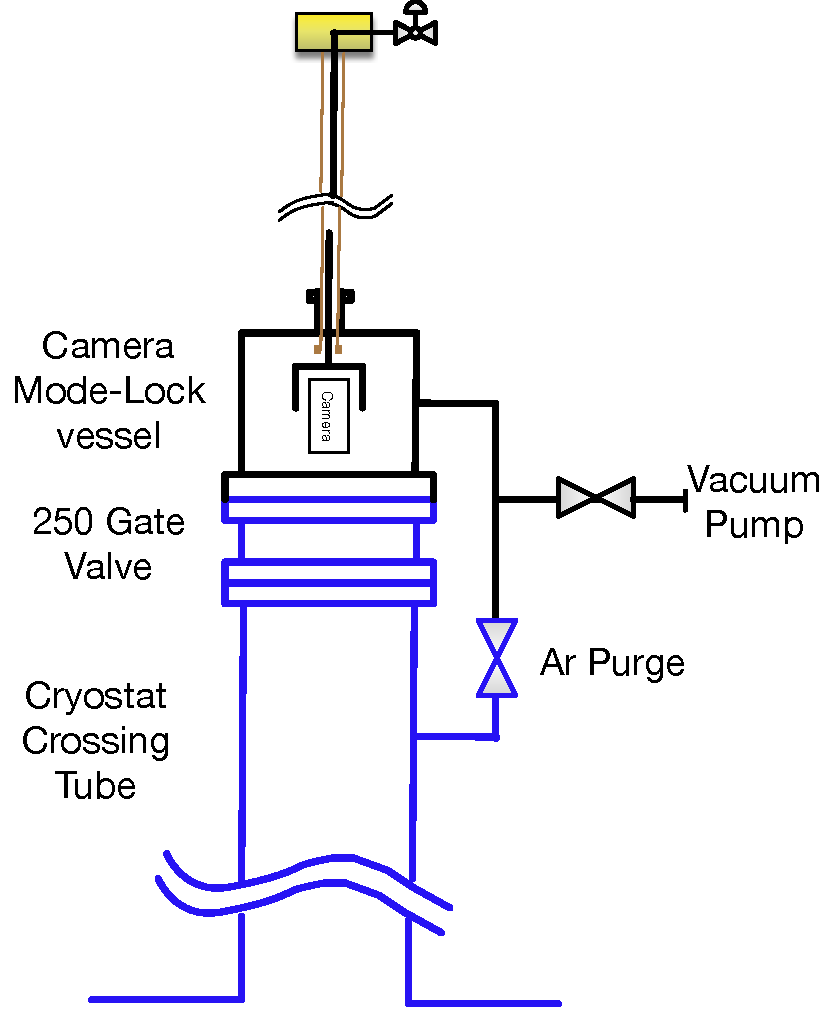
\includegraphics[width=0.3\textwidth]{Camera-Sketch}%
\end{dunefigure}

The design for the inspection camera system employs the same basic
enclosure design as for cold cameras, but mounted on an insertable
fork using a design similar to the dynamic temperature probes. (See
Figure~\ref{fig:gen-fdgen-cameras-movable} and
Figure~\ref{fig:fd-slow-cryo-sensor-mount}.)  The entire system is sealed to
avoid contamination with air. In order to avoid contamination, the
camera can only be deployed through a \fdth equipped with a gate
valve and a purging system, similar to that used for the vertical axis
calibration system at \kamland~\cite{Banks:2014hra}. The entire system
is  purged with pure argon gas before the gate valve is opened.

Motors above the flange allow rotation and vertical movement of the fork. 
 A chain drive system, with motor
mounted on the end of the fork, allows tilting of the camera assembly, 
creating a point-tilt mount with vertical motion capability.
Taking into account the room above the cryostat flanges and the
thickness of the cryostat insulation, a vertical range of motion of
\SI{1}{m} inside the cryostat is achievable.
% In the event that it
% becomes necessary to deploy a camera more deeply, we would have the
% option of building a a cable deployment system or a multi-pole
% deployment system similar to the KamLAND full-volume calibration
% system\cite{Busenitz:2009ac}, but this is not currently part of the
% baseline design.
The motors for rotation and vertical motion are located outside the sealed
volume, coupled mechanically using ferrofluidic seals, thus reducing
contamination risks and allowing for manual rotation of the vertical
drive in the event of a motor failure.  A significant protyping and
testing effort is needed to finalize and validate this design.

% % % %
\subsubsection{Light-emitting system}
%%% same text as dual-phase
The light-emitting system is based on \dwords{led} with the capability of illuminating the interior with selected
wavelengths (IR and visible) that are suitable for detection by the
cameras.  Performance criteria for the light-emission system are based
on the efficiency of detection with the cameras, in conjunction with
adding minimal heat to the cryostat. The use of very high-efficiency
\dwords{led}  %assists with the goal of 
helps reduce heat generation; as an
example, one \SI{750}{nm} \dword{led} has a specification of
\SI{32}{\%} conversion of electrical input power to light.

While data on the performance of \dwords{led} at cryogenic temperatures is sparse,
some studies related to NASA projects~\cite{Carron:2017zzz} 
indicate that \dword{led} efficiency increases with reduced temperature,
and that the emitted wavelengths may change, particularly for blue \dwords{led}.
The wavelength changes cited would have no impact on illumination, however, since
in order  to avoid degradation of wavelength-shifting materials in the \dword{pds},
such short wavelength \dwords{led} would not be used.

\begin{dunefigure}[\dword{led} chain for illumination]{fig:gen-cisc-LED}
  {Suggested \dword{led} chain for lighting inside the cryostat, with
    dual-wavelength and failure-tolerant operation.}
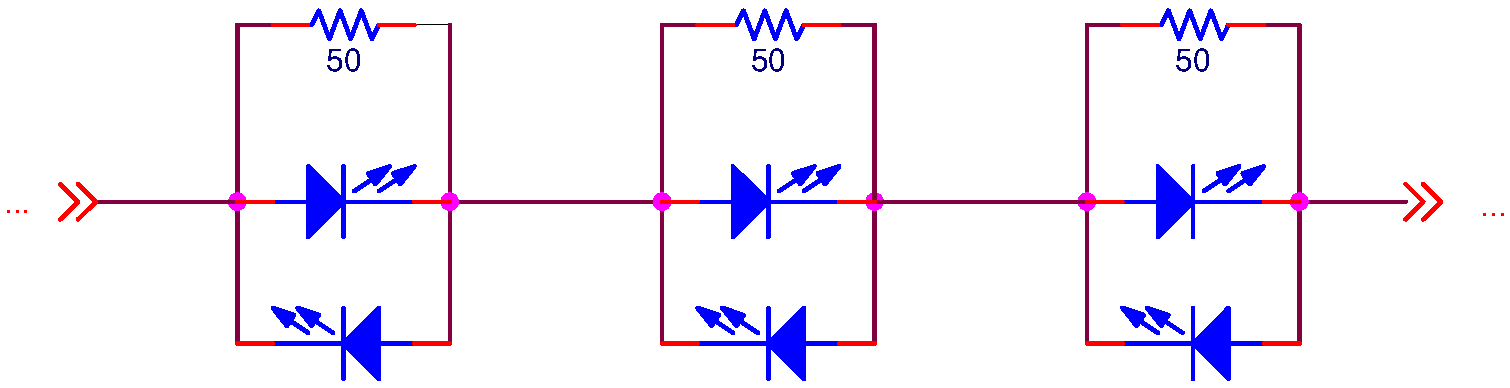
\includegraphics[width=0.7\textwidth]{CISC-Lighting}
\end{dunefigure}

\fixme{shoulds and woulds...}
A \textit{chain} of \dwords{led} should be connected in series and driven with a
constant-current circuit. It would be advantageous to pair each
\dword{led} in parallel with an opposite polarity \dword{led} and a resistor
(see Figure~\ref{fig:gen-cisc-LED}).
This allows two different wavelengths of illumination with a single installed
chain (by changing the direction of the drive current) and 
continued use of an \dword{led} chain even if individual \dwords{led} fail.

The \dwords{led} should be placed as a \textit{ring light} around the outside of each
camera lens, pointing in the same direction as the lens, to 
illuminate the part of the \dword{detmodule} within the field of
view of the camera. Commercially available \dwords{led} can be obtained with
a range of angular spreads, and can be matched to the needs of the
cameras without additional optics. 

